\section{Osmé cvičení}

\subsection{Příklad}
K automatu $M$, který je dán následující tabulkou, zkonstruujte regulární gramatiku $\mathcal{G}$, která generuje jazyk 
$L = L(M)$.


\subsection{Příklad}
Ke gramatice $\mathcal{G}$ typu 3 zkonstruujte konečný automat, který přijímá jazyk $L(\mathcal{G})$. Gramatika \\
${\mathcal{G} = (N, \{a,b\}, S, P)}$, kde $N={S,A,B}$ a pravidla jsou
\begin{align*}
    S &\rightarrow abA \mid aB\\
    A &\rightarrow aA \mid aaA \mid a\\
    B &\rightarrow bB \mid b
\end{align*}

\subsection{Příklad}
Je dán derivační strom v bezkontextové gramatice:

\[
\begin{tikzpicture} %TODO: change the design?
    \Tree [.$S$ [.$S$ [.$S$ $\varepsilon$  ] 
                      [.$B$ [.$B$ $b$ ] 
                            [.$A$ $a$ ] ] ] 
                [.$A$ [.$A$ $a$ ] 
                      [.$A$ $a$ ] ] ]    
\end{tikzpicture}
\]
\begin{enumerate}[a), noitemsep]
%\itemsep0em 
    \item Napište pravidla minimální CF gramatiky, ve které je to derivační strom. 
    \item Napište levou derivaci odpovídající tomuto derivačnímu stromu.
    \item Rozhodněte, zda je gramatika víceznačná.
\end{enumerate}

\subsection{Příklad}
Je dána bezkontextová gramatika $\mathcal{G} = (N, \Sigma, S, P)$, kde $N = \{S\}$, $\Sigma = \{+, \star, -, x, y\}$, 
pravidly
\[
S \rightarrow +SS \mid \star SS \mid - SS \mid x \mid y
\]
\begin{enumerate}[a), noitemsep]
    \item Nakreslete derivační strom, který má za výsledek slovo $w = + x \star - y x y$.
    \item Zkonstruujte levou derivaci slova $w$ odpovídající derivačnímu stromu z části a).
\end{enumerate}

\subsection{Příklad}
Navrhněte bezkontextovou gramatiku $\mathcal{G}$, která generuje jazyk $L = \{0^i 1^i 2^j; i,j \geq 0\}$. Zdůvodněte, 
proč gramatika $\mathcal{G}$ jazyk $L$ generuje.

\subsection{Příklad}
Ke gramatice $\mathcal{G}$ zkonstruujte nevypouštěcí gramatiku $\mathcal{G}_1$, pro kterou platí 
$L(\mathcal{G}_1) = L(\mathcal{G}) - \{\varepsilon\}$.
\begin{align*}
    \mathcal{G}: S &\rightarrow aSbA \mid \varepsilon\\
    A &\rightarrow aBbA \mid bCB \mid CD\\
    B &\rightarrow bbBa \mid aS\\
    C &\rightarrow aAaA \mid \varepsilon\\
    D &\rightarrow SC \mid aABa
\end{align*}
